	\section{Cancer and polyps}
	  \subsection{What we are looking for REM}
	  Different types of disorders.
	  %TODO image of polyp
	  Polyp is harmless, but if left untreated it can become cancerous
	  %TODO tell the risk
	  Pictures is from the pillcam project, kvasir dataset.
	  \subsection{images from pillcam, and what we are looking at/for REM}
	  %TODO More pictures of polyps, and other anomalies
	  
	
	\section{Naive Methods REM}
	  Now that we have an idea of what we are looking for we can first turn to some more naive methods for detecting anomalies, and for enhancing the images.\\
	  The field of image processing has been researched since\\ %TODO WHEN
	  
	  Using some of the classic methods in image processing we can see if\\ %TODO
	  
	  We often describe the method in to two groups of information: First and Second order statistics.\\
	  \textbf{First order:} First order statistics does not take in to account the relative positioning of the pixels in the image, and because of this, gives much less
	  information than the second order statistics.\\
	  Example of First order statistics is often what information we can get out of a histogram. This can be scewness, variance, and mean value.\\
	  
	  \vspace{10px}
	  
	  \textbf{Second order:} Second order statistics takes in to account the relative positioning of the pixels in the image. We can calculate the GLCM matrix and get a much more detailed 
	  view of the image. \\
	  
	  
	  
	  \subsection{GLCM}
	    A GLCM (Grey-level co-occurrence matrix) is a matrix that is used when examining the spatial relationship of pixels in a texture. 
	    The calculation of a GLCM gives us how often pairs of pixels with spesific values and a specified spatial relationship occur at a given place in an image. %TODO CITE
	  
	    \subsubsection{Algorithm}
	      For simplicity we use only greyscale in this example:
	      \begin{figure}[ht]
		\centering
		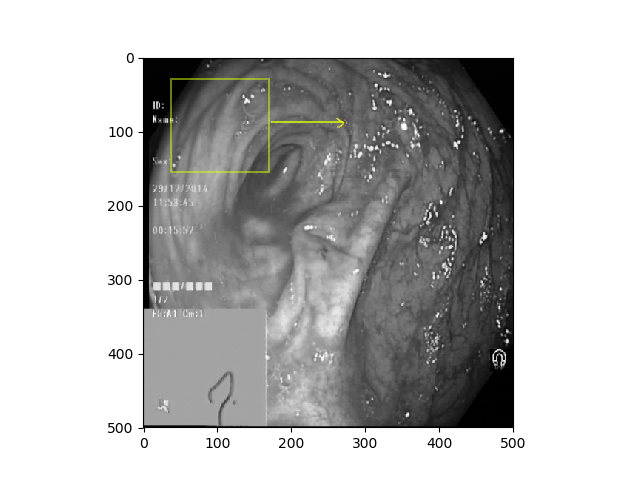
\includegraphics[scale=0.5]{figures/sliding_window_box.png}
		\caption{GLCM capturing features}
	      \end{figure}
	      The algorithm starts by running a sliding window over the image, often with a stride, and for each stops calculates the spatial relationship between each pixel specified.
	      The result can be something like this figure %TODO link to figure
	      where we can read out the most likely neighbouring pixel.
	       \begin{figure}[ht]
		\centering
		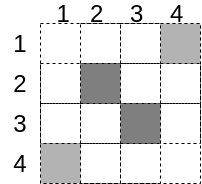
\includegraphics[scale=0.5]{figures/Simple_GLCM.png}
		\caption{GLCM Matrix}
	      \end{figure}
	      The darker colours on in the matrix is indicating that we often have a jump between, for instance pixel-value of 1 and a pixel-value of 4, but no from 1 to 1.\\
	      With this information we can get a naive pattern-recogniser. 
	    \subsubsection{Other uses}
	      Besides for the pattern recognition we can use the GLCM to get the information on:
	      \begin{itemize}
	       \item \textbf{Contrast} is the difference in luminance or colour in the picture. We would expect low contrast in the “background” and higher contrast around edges and irregular objects.
	       \item \textbf{Homogeneity} is how similar a local area is to itself
	       \item \textbf{Variance} $\sigma^2$ , is directly a measure of ”roughness”
	       \item \textbf{Mean} value of a GLCM can give us areas with higer or lower pixel values. Good way to find polyps if they are lighter than the tissue around.
	       \item \textbf{Entropy}
	       \item \textbf{Energy}
	      \end{itemize}


	  
	  \subsection{Edge detection}
	    Using Edge detection in is another viable way to look for polyps. 
	    \begin{figure}[ht]
	      \centering
	      \begin{minipage}[b]{0.45\textwidth}
		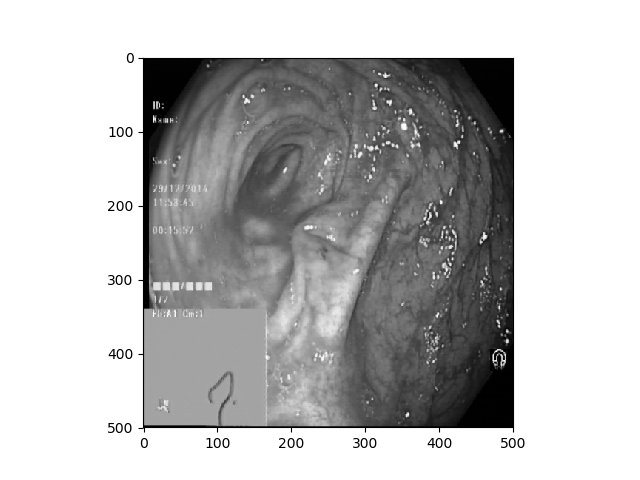
\includegraphics[width=\textwidth]{figures/sliding_window.png}
		\caption{Original image}
	      \end{minipage}
	      \hfill
	      \begin{minipage}[b]{0.45\textwidth}
		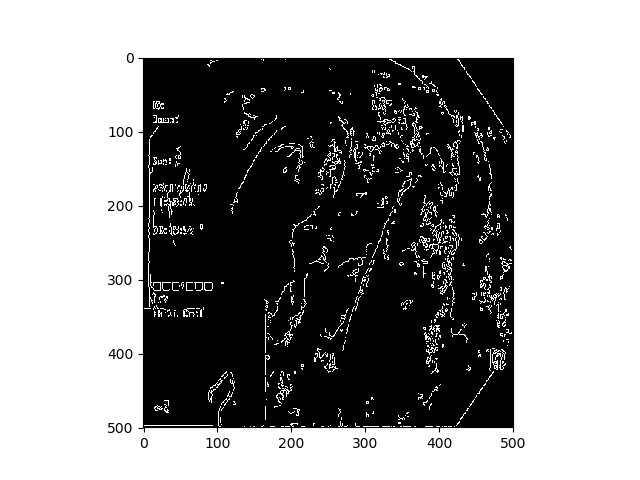
\includegraphics[width=\textwidth]{figures/Canny.png}
		\caption{Edges of the picture}
	      \end{minipage}
	    \end{figure}
	    \subsubsection{Algorithm}
	      For each pixel look at the neighbouring pixel, if \\
	      
	      \begin{centering} 
		$ abs(p_a - p_b)>tresh $\\ 
	      \end{centering}
	      
	      then mark pixel as an edge pixel. \\
	      
	  \subsection{Hough Transforms}
	    Using for instance Canny edge detection %TODO CITE
	    we can get a better view of where the potential border of the polyp/anomaly is. (As shown in %TODO FIG CITE)
	    
	    A hough transform can i theory have many/any shape(s), and together with edge detection, we might find some of the polyps this way.
	    
	    
	  
	  
	\section{Machine Learning}
	Machine learning is a very broad term, but can i short be summarised by:\\
	\vspace{10px}
	
	\textit{ A computer program is said to learn from experience E with respect to 
	some class of tasks T and performance measure P, if its performance at
	tasks in T, as measured by P, improves with the experience E. } 
	\cite{MitchellTomM1997Ml}\\
	
	\vspace{10px}
	Here we have a couple of parameters:\\
	\textbf{E} text about e\\
	\textbf{T} text about t\\
	\textbf{P} text about p\\
	
	From this we see that the goal of machine learning is to improve some performance P with experience.
	\textbf{might here talk about different tasks ML can do?}
	
	  \subsection{Supervised \& Unsupervised machine learning}
	  We often divide machine learning in to two (diffuse) categories: supervised and unsupervised.\\
	  
	  \vspace{5px}
	  \textbf{Supervised learning:} is the act of training with data that has an answer or a label. The learning algorithm can get supervision while 
	  training on the task. An example on a supervised task  is to recognise handwritten numbers, or differentiate between dogs and cats. The task is supervised if the images
	  comes with the correct label in the data set. These  examples are typical classification examples, where the task is to identify the right group to classify the data to %TODO more
	  A simpler classification assignment is binary classification, where the target is (often) yes or no. Examples for binary classification is if an email is spam or not, is a car Norwegian 
	  or International. 
	  In the last example the classification changes from binary to multi-class if you sort the cars on every nationality, and not just Norwegian/non-Norwegian.
	  
	  Another type of supervised learning is regression. This is the act of prediction given prior data. Examples of regression is everything from prediction of stock prices, to house prices 
	  in an area, to\\ %TODO more
	  \begin{figure}
	     \centering
	    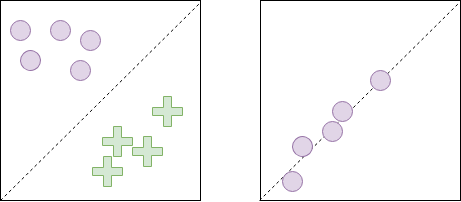
\includegraphics[scale=0.5]{figures/class_vs_reg.png}
	     \caption{Left: Example of binary classification. Right: Example of regression} 
	  \end{figure}

	  
	  \vspace{5px}
	  \textbf{Unsupervised learning:} is the act of training without any supervision, on the sense that we do not give the algorithm the answer
	  to the training data set. %TODO more 
	 
	  Since we do not have categorised data in unsupervised learning, we often %TODO more
	  Types of unsupervised learning can for instance be clustering, the act of sorting data based on similarity. An example of this can be if you want to sort plants based on species, or 
	  you are detecting anomalies in a dataset.
	  Unsupervised learning can be used for PCA %TODO CITE 
	  or other dimensionaly reduction methods.\\
	  
	  A third method to used unsupervised learning is the adversarial route, where you use machine learning to make similar looking data to the original data set. 
	    
	   \begin{figure}
	     \centering
	    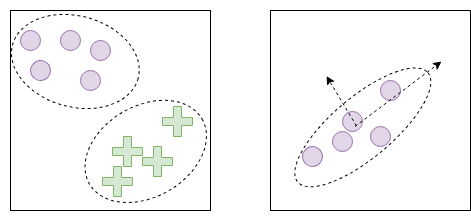
\includegraphics[scale=0.5]{figures/cluster_pca.png}
	     \caption{Left: Example of binary clustering. Right: Example of principal component analysis} 
	  \end{figure}

	 
	  In the description of supervised vs unsupervised we looked at a specific branch of machine learning: Classification. Classification is, as the name implies, the task of 
	  getting data sorted in to groups of similarity. 
	  
	  
	  \begin{itemize}
	    \item subsfication
	    \item r to the pillcam projression 
	    \item transcription/translation
	    \item de-noising /finding missing inputs
	  \end{itemize}
	  
	  \subsection{Types of machine learning}
	  There are a number of different machine learning algorithms. %TODO tell that we are going inn to detail here
	  \begin{table}[ht]
	    \centering
	    \resizebox{\textwidth}{!}{%
	    \begin{tabular}{|c|c|c|c|c|}
	      \hline
	      \multicolumn{5}{|c|}{Machine Learning}                                                                                 \\ \hline
	      \multicolumn{2}{|c|}{Supervised Learning}   & \multicolumn{2}{c|}{Unsupervised Learning}       & Reinforcement Learning\\ \hline
	      Classification          & Regression        & Clustering           & Dimensionality reduction  & -                     \\ \hline
	      Support vector machines & Linear Regression & K means clustering   & PCA                       & SOMething             \\
	      K nearest neighbours    & Decision trees    & Hidden Markov models &                           &                       \\
	      Neural networks         & Neural networks   & Neural Networks      &                           &                      
	    \end{tabular}%
	    }
	    \caption{Machine leaning types}
	    \label{ML-types}
	  \end{table}
	  
	  %TODO rewrite under.
	  
	  \vspace{5px}
	  \textbf{K nearest neighbours}\\
	  Talk about KNN\\
		 
	  \vspace{5px}
	  \textbf{Linear Regression}\\
	  How to regress linearly\\
	  
	  \vspace{5px}
	  \textbf{Support vector machine}\\
	  SVM and 2 class\\
	  
	  \vspace{5px}
	  \textbf{Others?}\\
	  Other important ones to talk about?\\
	  
	  
	  \vspace{5px}
	  \textbf{Neural networks}\\
	  %TODO har given good results last years
	  %leading in the field
	  %own chapter
	  NN is future\\
	  own chapter\\
	  
	
	\section{Neural Networks}
	  
	  
	  \subsection{How it works}
	    %TODO talk about backward/forward prop?
	    %
	
	  
	  \subsection{Convolutional neural networks}
	  
	  \subsection{Advaserial neural networks}
	  
	  
	  
	  \subsubsection{UCNN?}
	  
	  
	  
	\section{The problem at hand}
	  Now that we have the definition of machine learning we focus on the task at hand; finding polyps. In an ideal world we have a
	  Classification problem with only two classes: Non-polyp and polyp. 
	  
	  \begin{itemize}
	    \item SVM 
	    \item CNN 
	    \item random forests
	    \item knn
	  \end{itemize}
	  
	
	\section{In painting}
  We have discussed the importance of good input data, and the potential benefits to resource usage and ease of making a good model.
  So a priority when it comes to image classification is to have data without anomalies and other areas that can be interpreted as a feature for the classifier. 
  In a machine learning perspective, the data is best if it has the same structure, and is %TODO similar enough.
  In painting is the process of reconstructing lost or deteriorated parts of images and videos. %TODO CITE https://en.wikipedia.org/wiki/Inpainting
  

  From prior papers on polyp detection in the GI tract %TODO CITE!!!
  we have clear results that the black corners, and the green squares trigger a big activation %TODO WRITE BETTER
  when it comes to classifying images. 
  From %TODO CITE, find out who
  's paper, we can see that the activation map on a regular image gives very high result on, in addition to the polyp, the corners and the green sqare. 
  \begin{figure}[ht]
    \centering
    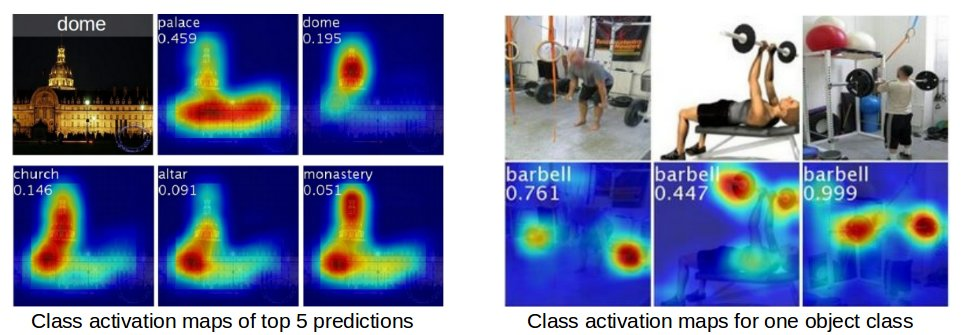
\includegraphics[scale=0.5]{background/figures/placeholder.jpeg}
    \caption{Using X's activation map we can see that the edges triggers unwanted activations}
  \end{figure}
  
  In addition to sqares and edges, we also have the problem that parts of the image is over saturated at points where the light from the led is reflected directly back to the camera.
  Another problem is when the camera captures images that are too close to the wall. Both of these scenarios creates patches where the saturation is maximum. 
   \begin{figure}[ht]
    \centering
    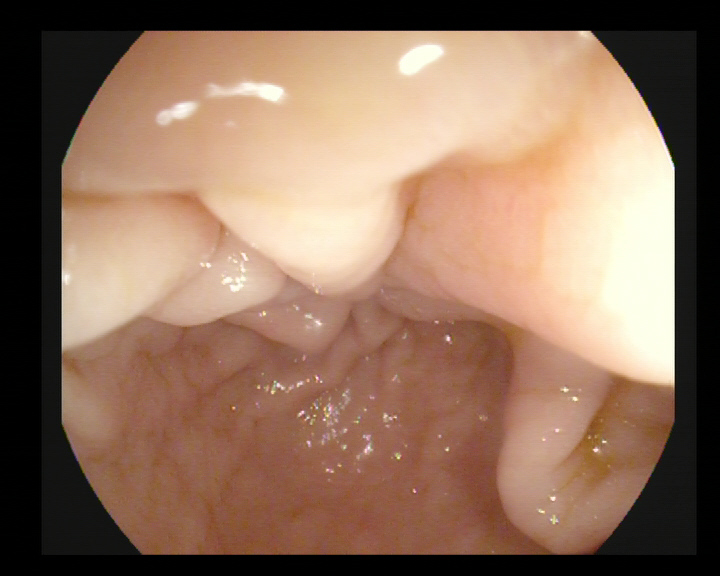
\includegraphics[scale=0.5]{background/figures/reflection.jpg}
    \caption{we have two different types of saturation: the reflected area in the top part of the image, and the right side of the image.}
  \end{figure}
  in an ideal scenario the image would have no pixel values at max, and as little frame as possible. 
  We therefor want to make a tool that can help us with this.
  \subsection{Naive methods for In painting}
    Inpainting is not a new area of research, as it has been around since %TODO CITE
    Because of this there are many naive methods that gives good inpaintings. 
	
    \subsubsection{Textured syntesys based on image inpainting}
    \subsubsection{MOARE}
    \subsubsection{MOARE}
	
    As we can see from this, there are a lot of old methods that can give approximations. We can also conclude that none of these methods are perfect.
    We will therefore look at methods that takes learning in to use.
  \subsection{Using machine learning for inpainting}
    As discussed earlier, machine learning is using prior experiences to make decisions given the problem at hand. 
    It is also worth mentioning that we do not need labeled data, since we are in a way looking at a global average of every image both with, and without polyps. We are therefor insetiviced to use an 
    Unsupervised approach.
    Since machine learning is learning from a training set, it is important that the training set contains as little as possible of the features we want to remove. \\
    
    Because of this the first thing we need to do if we are going to mask out corners and sqares, is to limit the training set to only contain cropped, non-sqare images. 
 
    \begin{figure}[ht]
      \centering
      \begin{minipage}[b]{0.45\textwidth}
	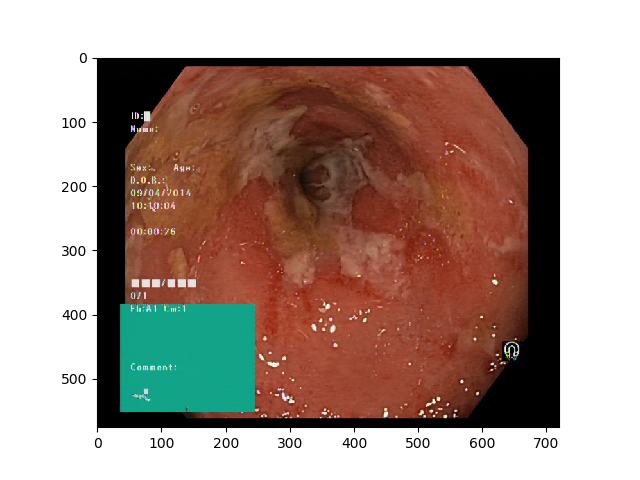
\includegraphics[width=\textwidth]{background/figures/uncropped_img.png}
	\caption{Original image with black padding}
      \end{minipage}
      \hfill
      \begin{minipage}[b]{0.45\textwidth}
	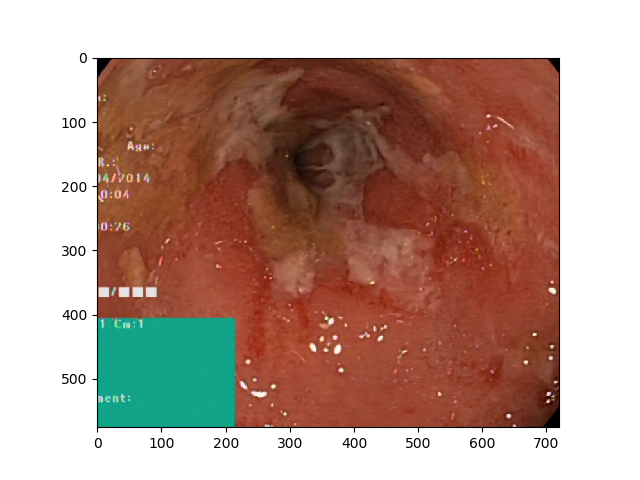
\includegraphics[width=\textwidth]{background/figures/cropped_8percent_img.png}
	\caption{Black edges cropped away + 8\% zoom}
      \end{minipage}
      \caption{Here we have an example on how we would make an image better to train on. This is not representative of the training, since we only use images without the green square under training}
    \end{figure}
    
    Now that we have better images to train our data with, we need the correct algorithm.
    We have already seen unsupervised learning aproaches in chapter %TODO ref 
    \newpage
    \subsubsection{Algorithm}
      \todo{Hvordan skal jeg gaa frem nar det kommer til aa presantere disse? skal jeg bare si hvilke metoder jeg har testet?}
      Text about presenting UML, and stuff.
      \subsubsection{Autoencoder}
	\paragraph{This is explaining Autoencoders, put me in the right place} %%TODO CITE: http://www.deeplearningbook.org/contents/autoencoders.html
	  As we recall from earlier, an autoencoder is a type of neural network that tries to output a recreation of the output.\todo{we are not recalling} \\ 
	  We can do this by having an encoder, $h=f(x)$, connected to a decoder, $r=g(h)$. 
	  An autoencoder has the job to set $g(f(x))=x$ over the whole input, but in most cases this is not a practical program. We often gives the autoencoder the restriction
	  that it has to map the input through a latent space that has a smaller dimension than the input dataset.\\
	  This is called an undercomplete autoencoder.\\
	  \vspace{10px}
	  \begin{figure}[ht!]
	    \centering
	    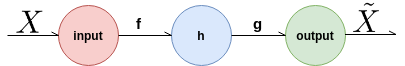
\includegraphics[scale=0.5]{background/figures/SimpleAE.png}
	    \caption{The general structure of an autoencoder, mapping $\textbf{x}$ through $\textbf{h}$ to an output $\textbf{r}$.}
	  \end{figure}
	  
	  As with supervised classifiers we can use gradient decent to optimize the model. This is because we are trying to recreate the input $\textbf{x}$ from out output $\widetilde{\textbf{x}}$\\
	  
	  This can simply be done by minimizeing the loss function\\
	  \begin{equation}
	    L(\textbf{x},g(f(\textbf{x})))
	  \end{equation}
	  with for instance MSE with gradient decent. \todo{explain MSE, and general loss on an ealier time}\\
	  
	  Now we can transfer this to a more relevant example by making an image as input and use convolutions to reduce the dimensionality in the encoder and increase the dimentionality in the encoder.
	  \vspace{10px}
	  \begin{figure}[ht!]
	    \centering
	    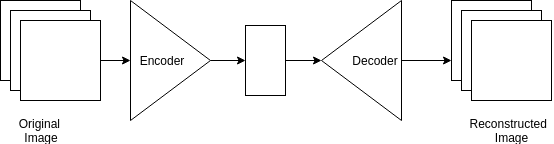
\includegraphics[scale=0.5]{background/figures/CAE.png}
	    \caption{Convolutional autoencoder with an RGB image as input, and the reconstructed image as output.}
	  \end{figure}
	
	\newpage
	test
	
	
	\newpage
	As we recall from earlier, an autoencoder is a type of neural network that tries to output a recreation of the output.\\%TODO: REF the part about autoencoders 
	We can use this for inpainting by setting the algorithm to train on images with areas cropped away.
	There are a couple of different way we can train an autoencoder to do this.\\
	
	%\todo{should i talk about the different ways or present the best?}
	
	
	\vspace{10px}
	\textbf{Denoising Autoencoder with MSE loss:}\label{par:Denoising_Autoencoder_with_MSE_loss}\\
	The simplest way to train the autoencoder is to first take the trainingset $\mathds{X}$ and make an augmented copy $\widetilde{\textbf{x}}^{(i)}$ for 
	every data point in $\textbf{x}_{\sim \mathds{X}}^{(i)}$. \\
	\textit{Here $\widetilde{\textbf{x}}$ is a copy of x with random areas masked.}\\
	
	Now we minimize the loss function\\	
	  \begin{equation}
	    L(\textbf{x},g(f(\widetilde{\textbf{x}})))
	  \end{equation}
	over the whole image.\\
	\vspace{20px}
	
	With this approach the autoencoder learns to fill in the blank spots with plausible data, without changing the rest of the image. 
	\todo{this will probably work best if the autoencoder is not undercomplete, perhaps talk about this}
	One problem by this approach is that we do not want the rest of the image to change for obvious reasons, and the alogrithm as it is here has the flaw that it will change all the pixels in the image, at 
	least to a minor degree. \\
	
	This can be somewhat fixed by only taking the augmented parts, and pasting the directly in to the image. This will leave most of the original image, except for the parts that was cropped randomly.\\
	
	\vspace{10px}
	\textbf{Denoising Autoencoder with \todo{clever tittle}:}\\
	If we take what we learned from \ref{par:Denoising_Autoencoder_with_MSE_loss}, we can make a more optimal autoencoder:
	Rather than taking a loss like 	
	\begin{equation}
	  L(\textbf{x},g(f(\widetilde{\textbf{x}})))
	\end{equation}
	over the whole image, we can rather just focus on the parts that matters, namely the cropped areas.\\
	
	If we add the cropped image to the output from the autoencoder to make an image image, we can use this new image to train out loss.
	For most of the image, the loss will be zero, since the only part that is changed is the cropped area. 
	We can also make a new loss that is more optimal for the task at hand. 
	\begin{equation}
	  MSE_{crop}\:=\: \frac{1}{n}
	  \begin{cases}
	      \begin{array}{lcl}
	      (\widetilde{\textbf{x}}-\textbf{x}) \; if \; \widetilde{\textbf{x}} \: \in \: \textbf{x}_{crop} \\
	      0 \; else
	      \end{array}
	  \end{cases}
	\end{equation}
	Where $\textbf{x}_{crop}$ is the area that was cropped away from the original image and $n$ is the number of pixels in that area.\\
	With this modified MSE we are assured that only the pixels in the cropped area is changed with gradient decent, and we save a lot of computation as an added bonus.
	
	
	\todo{token to not train}
	\begin{figure}[ht!]
	    \centering
	    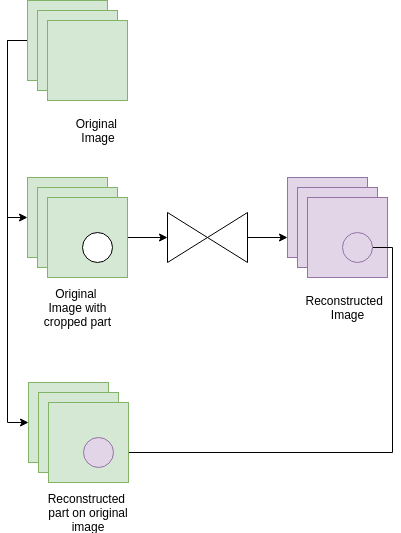
\includegraphics[scale=0.5]{background/figures/AE_for_inpainting.png}
	    \caption{Final result of the autoencoder used in the testing}
	\end{figure}
	
	
	
	
	

      \subsubsection{Contextencoder}
      \subsubsection{CCgan}
      \subsubsection{PixelCNN}
      
  
 
